\documentclass[runningheads]{llncs}

\usepackage[T1]{fontenc}
\usepackage[utf8]{inputenc}
\usepackage{graphicx}
\usepackage{booktabs}
\usepackage{multirow}
\usepackage{amsmath,amssymb}
\usepackage{array}
\usepackage{xcolor}
\usepackage{orcidlink}
\usepackage{url}
\def\UrlBreaks{\do\/\do-\do_}
\usepackage{microtype}
\usepackage{caption}
\usepackage[section]{placeins}
\usepackage{cite}
\usepackage{hyperref}
\hypersetup{colorlinks=true, linkcolor=blue, citecolor=blue, urlcolor=blue}

\newcommand{\CQ}{CycleQA}

\begin{document}

\title{Cross-Vendor Quality Assurance of Zero-Shot Full-Cycle 4D Cardiac Cine MRI
Segmentation via Dual-Anchored Medical Video Foundation Model}
\titlerunning{Cross-Vendor Quality Assurance of Zero-Shot Cine CMR Segmentation}

\author{Zhuoan Li\orcidlink{0009-0005-0647-8579}}
\authorrunning{Z. Li}
\institute{Weldon School of Biomedical Engineering, Purdue University,
           West Lafayette, IN, USA\\
           \email{li4533@purdue.edu}}

\maketitle
\begin{abstract}
Reliable quality assurance remains a barrier to deploying zero-shot foundation models for cardiac image segmentation, because performance may deteriorate across scanner manufacturers and reference masks are unavailable to identify failures. We introduce \CQ{}, a prediction-only framework for detecting and mitigating failures in full-cycle cine cardiac magnetic resonance segmentation. A fixed dual-anchored medical video foundation model based on MedSAM2 is initialized separately at the clinically defined end-diastole (ED) and end-systole (ES) frames, with each anchor propagated across the entire cardiac cycle to produce two full-cycle segmentations. \CQ{} uses disagreement between the ED- and ES-anchored predictions as an intrinsic measure of segmentation reliability. The framework was developed on 100 ACDC patients and evaluated without adaptation on 320 M\&Ms patients from four scanner manufacturers, five centres, and nine pathology groups. Under external validation, mean absolute left ventricle ejection-fraction (EF) error increased from 6.4 to 23.4 percentage points (pp), while the proportion of studies containing at least one failed structure increased from 11\% to 54\%. Without reference masks, vendor information, retraining, or test-time adaptation, propagation disagreement estimated external Dice with a mean absolute error of 0.072 ($R=0.814$) and detected failed studies with an AUROC of 0.850 (95\% CI 0.811--0.888). Performance remained robust on Canon examinations absent from development (AUROC 0.806), whereas an appearance-based out-of-distribution detector achieved 0.573. Risk-guided selection among the ED-anchored, ES-anchored, and dual-anchored segmentation reduced EF error from 23.4 to 12.0 pp and the failure rate from 54\% to 15\%, without additional inference. These results demonstrate that propagation disagreement provides an actionable, label-free quality-control signal for cross-vendor deployment. Code is available at  \url{https://github.com/zhuoanli/CycleQA}

\keywords{Medical video foundation model  \and Quality assurance \and Failure detection \and Cross-vendor validation}
\end{abstract}

\section{Introduction}
Promptable medical video foundation models have made zero-shot segmentation of dynamic medical imaging increasingly feasible \cite{ravi2024sam2,zhu2024medsam2}. In cine cardiac MRI, this capability can be extended across the full cardiac cycle through dual-anchored propagation. MedSAM2 is initialized separately using bounding-box prompts at the clinically defined ED and ES phases, and each anchor is propagated across the complete sequence to produce an ED-anchored and an ES-anchored segmentation trajectory. The two trajectories are subsequently merged to obtain a full-cycle segmentation. Because this approach requires neither cardiac-specific training nor site-specific model adaptation, it is particularly attractive for clinical settings in which densely annotated local datasets are rarely available.

This advantage, however, creates a related challenge: a model that can be deployed without target-domain training annotations is typically used without reference masks for verifying its predictions. Benchmark performance is measured where annotations are available, whereas clinical deployment occurs where they are not. Moreover, the benchmark itself may represent only a narrow imaging domain. ACDC \cite{bernard2018acdc}, on which the upstream segmentation system was developed, contains data acquired at a single centre using scanners from a single manufacturer. The resulting gap between benchmark performance and real-world generalizability remains a major obstacle to the clinical translation of imaging AI \cite{varoquaux2022failures,moor2023gmai}.

This study therefore addresses two questions. First, does the performance of a zero-shot cardiac video foundation model generalize across scanner manufacturers and clinical centres? We investigate this question using M\&Ms \cite{campello2021mnms}, an independent cohort of 320 patients spanning four manufacturers, five centres, and nine pathology groups. Second, and more importantly, can unreliable segmentations be identified at deployment when no reference mask is available?

Our approach exploits the redundant predictions generated by dual-anchored propagation. The medical video foundation model is initialized separately at the clinically defined ED and ES phases, with each anchor propagated across the complete cardiac cycle to produce an ED-anchored and an ES-anchored segmentation trajectory. Although the two trajectories share the same model and input video, their different anchor conditions and propagation paths provide complementary estimates of the underlying anatomy. Consistent tracking should produce similar segmentations, whereas anchor-sensitive drift should increase their disagreement. We therefore investigate inter-anchor disagreement as a prediction-only indicator of segmentation reliability and introduce \CQ{}, a quality-assurance framework for detecting and mitigating failures without reference masks. Our contributions are:

\begin{enumerate}
\item \textbf{Cross-vendor external validation.} Using 320 M\&Ms patients, we show that a moderate reduction in segmentation Dice can coincide with substantial degradation in clinically relevant measurements. Mean absolute EF error increases from 6.4 to 23.4 pp, demonstrating that Dice alone may understate the clinical effect of domain shift.

\item \textbf{Prediction-only quality assurance.} Without additional training, inter-anchor disagreement estimates segmentation Dice on the external cohort with a mean absolute error of 0.072 and detects failed studies with an AUROC of 0.850, including examinations from manufacturers absent during development. An appearance-based out-of-distribution control further shows that \CQ{} identifies segmentation error rather than merely recognizing the scanner manufacturer.

\item \textbf{Risk-guided intervention.} Without reference labels, retraining, or additional inference, \CQ{} uses the estimated risk to select among the ED-anchored, ES-anchored, and merged predictions already generated by the upstream system. In the external cohort, this approach reduced mean absolute EF error from 23.4 to 12.0 pp and achieved lower error than the fixed-selection strategies evaluated in this study.
\end{enumerate}


\section{Related Work}

\subsection{Promptable foundation models for CMR.}

SAM \cite{kirillov2023sam} and its video successor SAM2 \cite{ravi2024sam2} were adapted to
medical data as MedSAM \cite{ma2024medsam} and MedSAM2 \cite{zhu2024medsam2}. Prompting
strategies for cardiac MRI have been studied for the static case
\cite{stein2023samcardiac,chen2025cinecmrsam}, and CineMA \cite{fu2025cinema} pretrains a
cardiac-specific foundation model. Beyond segmentation, cardiac foundation models have been
adapted to downstream perfusion analysis \cite{shahin2026adapting} and to automated study
classification \cite{li2026classification}. The dual-anchored propagation scheme audited here
is specified in full in Sect.~\ref{sec:system}; it requires no training and no architectural
change, only a second prompt.
\vspace{-0.4cm}

\subsection{Domain shift in cardiac MRI}
Cross-vendor generalisation remains a well-documented challenge in supervised CMR segmentation \cite{tao2019multivendor,chen2020generalizability}. These limitations motivated multi-centre benchmarks such as the M\&Ms challenge \cite{campello2021mnms,martinisla2023mnm2}, while related work has shown that demographic imbalances in training data can introduce measurable performance disparities \cite{puyolanton2021fairness}. Zero-shot foundation models reduce reliance on task-specific annotated datasets, but they do not necessarily eliminate domain shift. Their learned representations still reflect the composition of the pretraining data, and differences in scanner manufacturer, acquisition protocol, and image appearance may affect downstream performance. Our cross-vendor evaluation examines whether such performance degradation persists without cardiac-specific training and shows that zero-shot deployment alone does not guarantee robust generalisation.
\vspace{-0.4cm}

\subsection{Segmentation quality control without ground truth}
Segmentation quality assessment without reference masks is an established area of research. Reverse Classification Accuracy (RCA) \cite{valindria2017rca,robinson2017qc} estimates segmentation quality by registering a predicted mask to an atlas database with known annotations. Other approaches train convolutional neural networks to regress quality scores directly \cite{robinson2019qc,tarroni2019qc,tarroni2020qc}, use generative shape priors \cite{wang2020genqc}, quantify ensemble disagreement \cite{hann2021qc}, or derive hand-crafted geometric descriptors \cite{kohlberger2012}. Quality-controlled cardiac analysis pipelines have also been deployed in large population studies \cite{ruijsink2020}. Model-intrinsic uncertainty provides another potential quality signal \cite{kendall2017uncertainties,lakshminarayanan2017ensembles,roy2019}, although its reliability for identifying individual segmentation failures remains variable \cite{jungo2019}. In cardiac MRI, uncertainty-guided analysis has been investigated for multi-centre and multi-field-strength perfusion segmentation \cite{yalcinkaya2024uncertainty}, and clinician-in-the-loop quality control has been applied to large registry cohorts \cite{yalcinkaya2024qc}. Appearance-based out-of-distribution methods \cite{hendrycks2017baseline,lee2018mahalanobis,gonzalez2022ood} instead identify unusual inputs, which is related to, but distinct from, determining whether the resulting segmentation is incorrect.

Three gaps are particularly relevant to zero-shot video foundation models. (i) most quality-control methods were developed for supervised, frame-wise segmentation networks \cite{robinson2019qc,tarroni2019qc,tarroni2020qc}, whereas video foundation models may accumulate errors during temporal propagation \cite{ravi2024sam2,zhu2024medsam2}. (ii) their reliability under frozen cross-vendor deployment remains insufficiently studied. (iii) existing approaches often require additional resources: RCA uses annotated atlases and per-case registration \cite{valindria2017rca,robinson2017qc}, supervised quality regressors require labelled development data, and ensemble methods require multiple models or inference passes \cite{hann2021qc,lakshminarayanan2017ensembles}. Appearance-based out-of-distribution detection identifies unusual inputs but does not necessarily indicate an incorrect segmentation \cite{hendrycks2017baseline,lee2018mahalanobis,gonzalez2022ood}.

\CQ{} addresses these gaps using the ED- and ES-anchored full-cycle predictions already generated by the dual-anchored segmentation system. Its training-free tier measures inter-anchor disagreement without an atlas, deployment-domain annotations, or additional inference. Its calibrated tier learns a study-level risk model on the development cohort and is then frozen for cross-vendor evaluation. In both tiers, segmentation quality is assessed from the predicted masks rather than scanner appearance.


\vspace{-0.3cm}
\section{Methods}
\vspace{-0.2cm}

\subsection{Overview and dual-anchored MedSAM2 segmentation system}
\label{sec:system}
\vspace{-1cm}

\begin{figure}[ht]
\centering
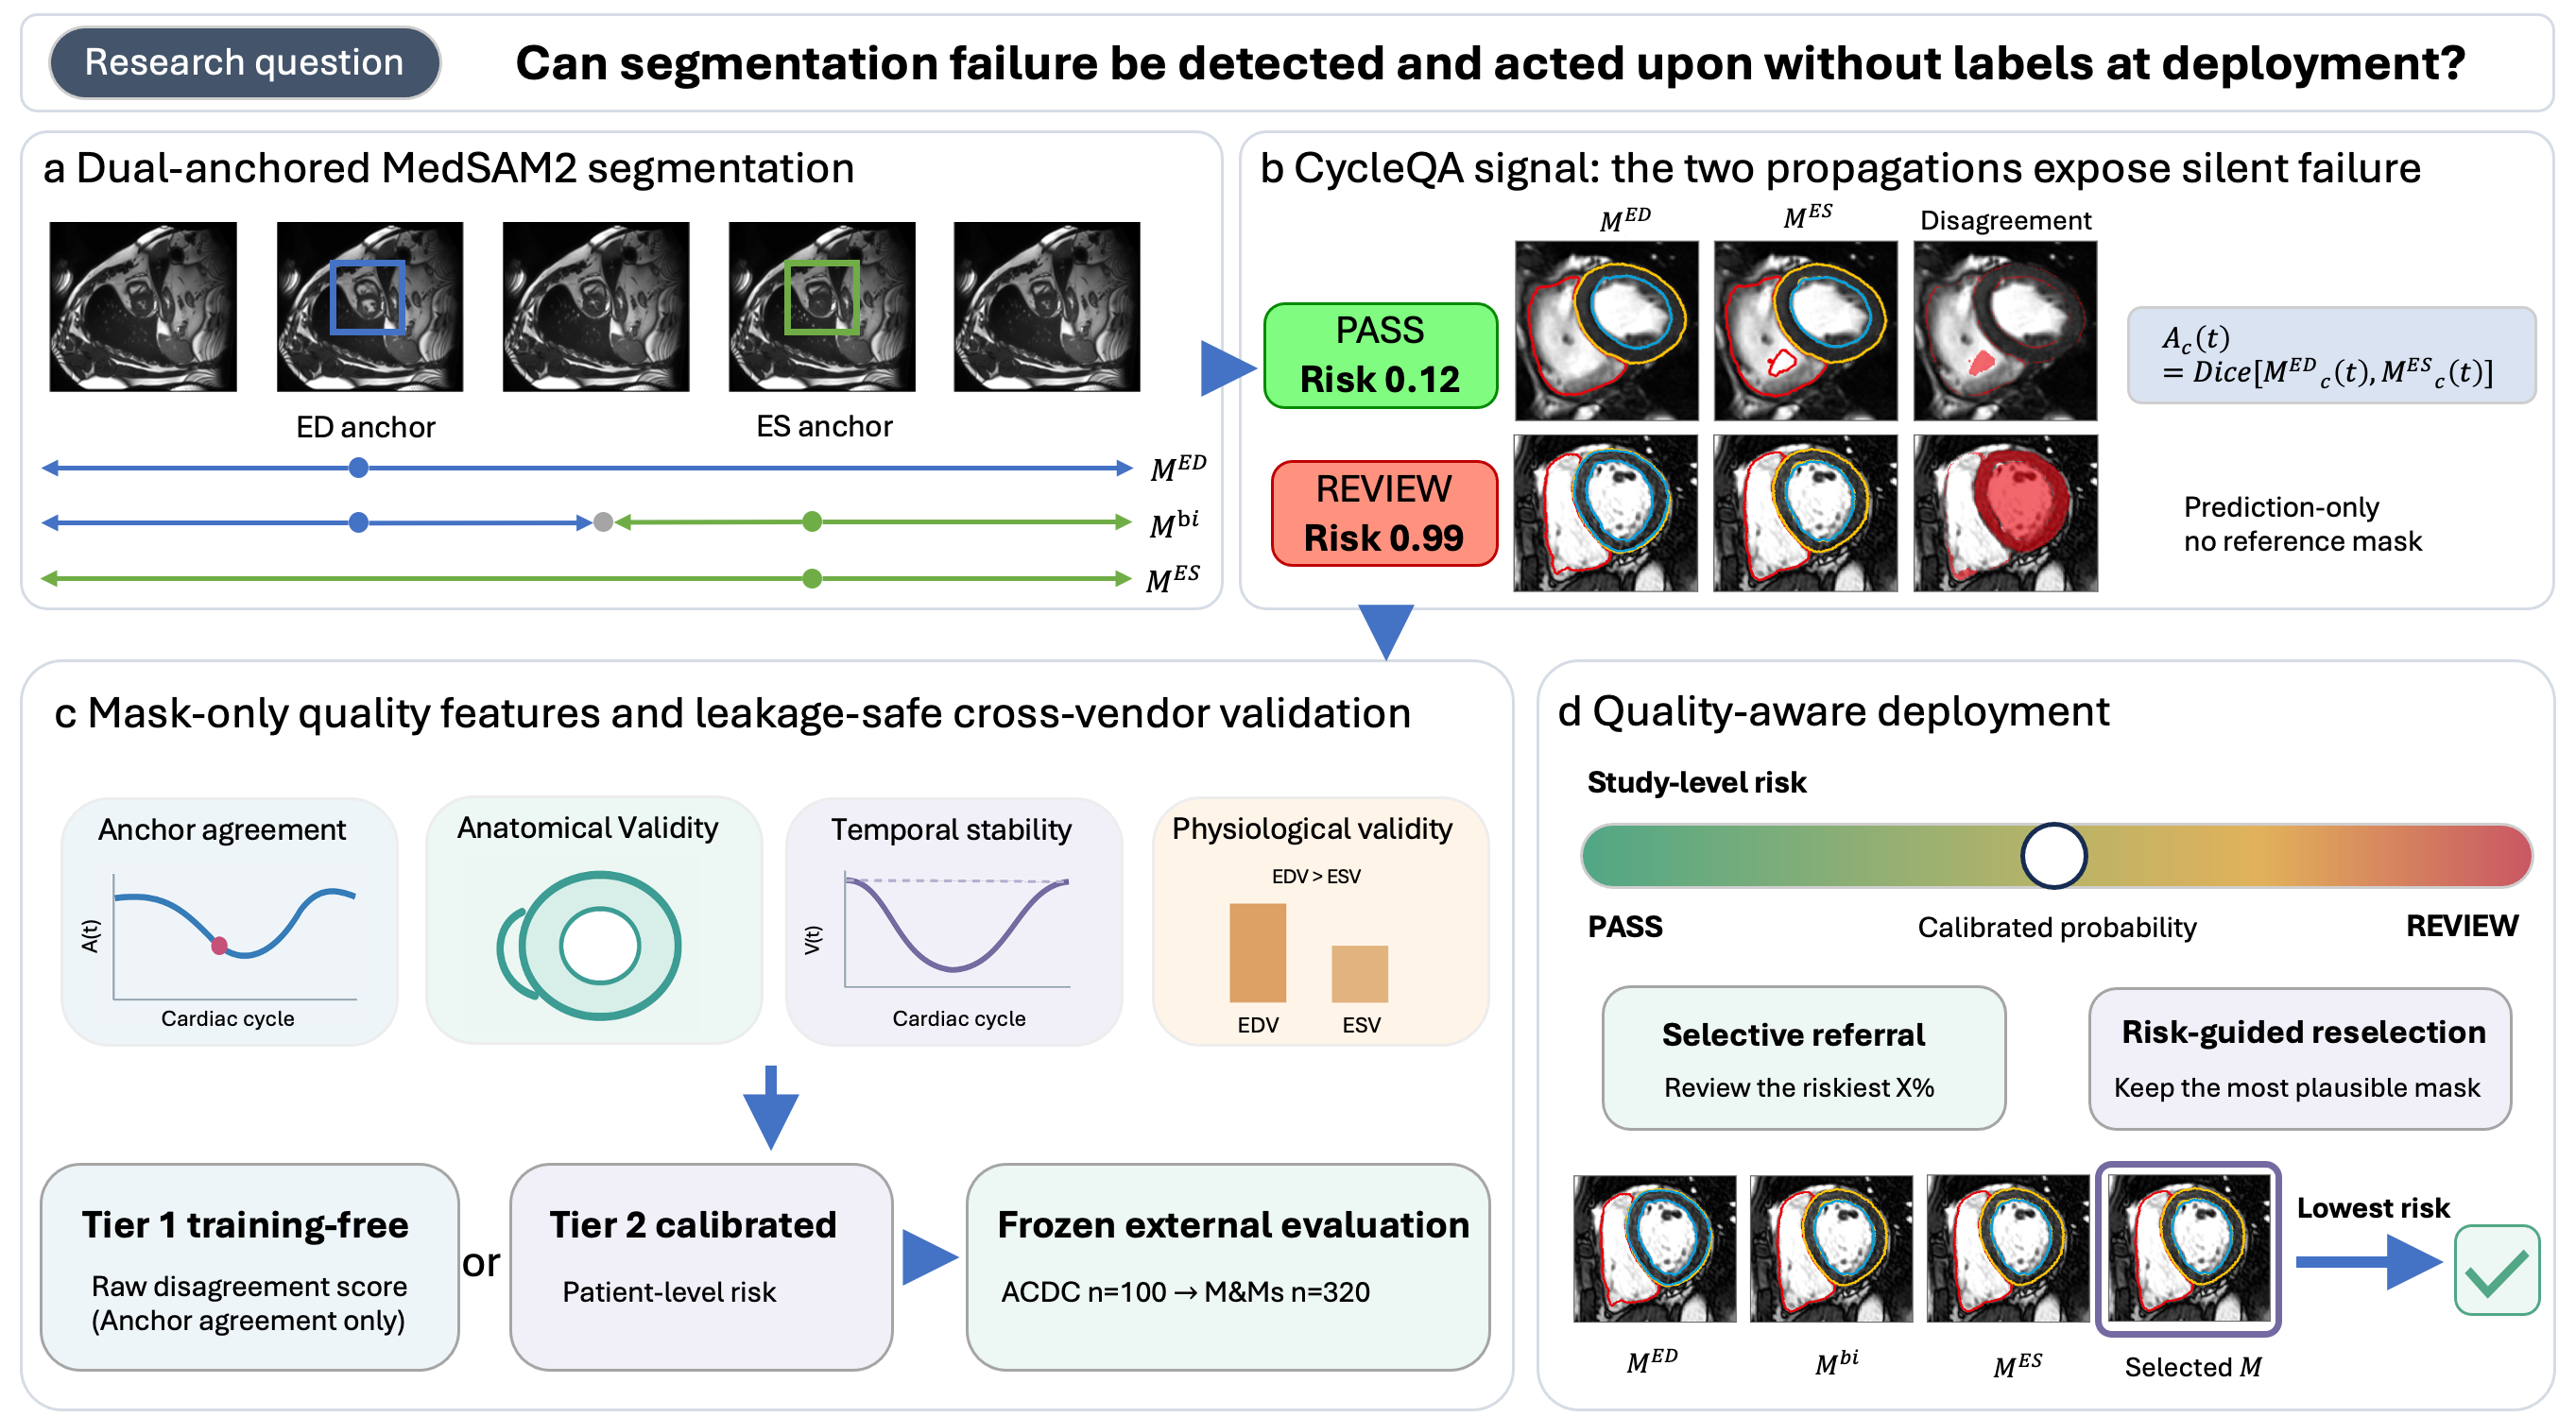
\includegraphics[width=\textwidth]{figures/method.png}
\caption{Overview of \CQ{}. a. Dual-anchored MedSAM2 segmentation. b. Inter-anchor disagreement. c.Mask-based quality and risk estimation. d.Quality-aware deployment.
}
\label{fig:overview}
\end{figure}

\vspace{-1cm}


Figure~\ref{fig:overview} summarises the \CQ{} framework. A fixed dual-anchored medical video foundation model first generates redundant full-cycle segmentations from ED and ES anchor frames. \CQ{} measures the consistency of these predictions, combines it with anatomical, temporal, and physiological descriptors, and produces a study-level quality estimate. The resulting risk can be used either to refer uncertain studies for review or to select among predictions already generated by the upstream system.

The segmentation system is based on MedSAM2 with a Hiera-tiny backbone and is treated throughout this study as a fixed upstream component. Each short-axis series is represented as a $2D+t$ sequence. MedSAM2 is initialized separately using bounding-box prompts at the clinically defined ED and ES phases, and each anchor is propagated across the complete cardiac cycle. This produces two full-length, anchor-conditioned predictions: $M^{\mathrm{ED}}$ and $M^{\mathrm{ES}}$. A third prediction, $M^{\mathrm{bi}}$, is formed using a nearest-anchor merge, in which each frame adopts the prediction associated with the temporally closer anchor. All three predictions are stored for subsequent quality assessment and reselection.


ED/ES box prompts were derived from reference masks; segmentation performance therefore represents an oracle-prompt upper bound. \CQ{} leaves the upstream segmenter unchanged, and automatic prompt generation is outside the scope of this study.


\subsection{\CQ{} quality features}

\CQ{} extracts 46 features exclusively from the predicted masks. Reference masks, true Dice scores, reference EF values, scanner manufacturer, centre, and pathology labels are excluded from the feature matrix. These exclusions are enforced during feature extraction to prevent information leakage.

The primary quality signal is inter-anchor agreement. For structure $c$ at cardiac phase $t$, we define

\begin{equation}
A_c(t)
=
\mathrm{Dice}\!\left[
M^{\mathrm{ED}}_c(t),
M^{\mathrm{ES}}_c(t)
\right].
\end{equation}

Because the two predictions are initialized at different physiological phases and follow different propagation paths, they may accumulate different temporal errors. High agreement indicates that the result is stable to anchor selection, whereas low agreement indicates anchor-sensitive inconsistency and suggests that at least one trajectory is unreliable. Agreement does not guarantee anatomical correctness, because both trajectories may converge on the same error; it is therefore combined with additional plausibility features.

The feature set comprises four families: anchor agreement (24 features), anatomical validity (6), temporal stability (8), and physiological validity (8). Agreement features summarise $A_c(t)$ using its mean, minimum, standard deviation, 10th percentile, mid-cycle mean, decay with distance from the anchors, and the proportion of frames below 0.7. Anatomical features describe containment, connectivity, and mask topology. Temporal features quantify volume-curve smoothness and cycle closure, while physiological features assess constraints such as ED volume exceeding ES volume. Table~\ref{tab:features} provides the complete feature definitions. All features are derived from predicted masks without reference masks or scanner metadata.

\begin{table}[t]
\centering
\caption{\CQ{} prediction-only feature families. }
\label{tab:features}
\small
\setlength{\tabcolsep}{4pt}
\renewcommand{\arraystretch}{1.12}
\begin{tabular}{@{}p{1.8cm}p{4.6cm}p{4.6cm}c@{}}
\toprule
Family & Descriptors & Rationale & $n$ \\
\midrule

Inter-anchor agreement &
Mean, minimum, standard deviation, 10th percentile and mid-cycle agreement; anchor-distance decay; fraction of frames with $A<0.7$ &
$A_c(t)=\mathrm{Dice}\!\left[M^{\mathrm{ED}}_c(t),M^{\mathrm{ES}}_c(t)\right]$. Agreement indicates stability to anchor selection, whereas disagreement reveals anchor-sensitive inconsistency. &
24 \\[2pt]

Anatomical validity &
Connected components; LV--myocardium containment; myocardial closure; LV holes; image-border contact &
Valid segmentations should preserve expected cardiac topology. Fragmentation, containment errors, holes and border contact indicate anatomically implausible masks. &
6 \\[2pt]

Temporal stability &
Inter-frame intersection over union (IoU); centroid displacement; volume-curve roughness; cycle closure, $|V(0)-V(T{-}1)|$; number of volume extrema &
Cardiac motion is temporally continuous and cyclic. Abrupt mask changes, irregular volume trajectories or incomplete cycle closure suggest propagation instability. &
8 \\[2pt]

Physiological validity &
$\mathrm{EDV}>\mathrm{ESV}$; EF-range violation; volume coefficient of variation; agreement between the annotated ES phase and the predicted volume minimum &
These descriptors provide weak physiological plausibility checks for the predicted volume trajectory and functional measurements. &
8 \\[2pt]

\midrule
\multicolumn{3}{@{}l}{\textbf{Total}} & \textbf{46} \\
\bottomrule
\end{tabular}
\vspace{-0.6cm}
\end{table}

\vspace{-0.4cm}

\subsection{Endpoints and evaluation protocol}
\vspace{-0.2cm}

Ground truth is used to define development targets and evaluate performance but is never included in the \CQ{} feature matrix. The primary endpoint is a failed study, defined as any cardiac structure with Dice $<0.70$ at an annotated ED or ES phase. The secondary endpoint is an absolute EF error greater than 10 percentage points:

\begin{equation}
|\Delta\mathrm{EF}_i|
=
\left|
\mathrm{EF}^{\mathrm{pred}}_i
-
\mathrm{EF}^{\mathrm{ref}}_i
\right|
>10~\mathrm{pp}.
\end{equation}

Both thresholds are specified before model evaluation and examined through sensitivity analysis, neither is selected to maximise AUROC. Because ACDC and M\&Ms provide reference segmentations only at ED and ES, these endpoints measure annotated-phase errors. Full-cycle predictions are used to derive the \CQ{} features, but intermediate frames are not treated as validated targets. We therefore do not claim direct evaluation of intermediate-phase failure detection.

\CQ{} is evaluated at two levels. \textbf{Tier~1} is training-free. For study $i$, inter-anchor agreement is averaged across all cardiac phases $\mathcal{T}_i$ and structures $\mathcal{C}=\{\mathrm{RV},\mathrm{Myo},\mathrm{LV}\}$:

\begin{equation}
\overline{A}_i
=
\frac{1}{|\mathcal{T}_i||\mathcal{C}|}
\sum_{t\in\mathcal{T}_i}
\sum_{c\in\mathcal{C}}
A_{i,c}(t).
\end{equation}

Mean agreement, $\overline{A}_i$, is used directly as an estimate of study-level segmentation quality, and its complement defines the training-free risk score:

\begin{equation}
r_i^{(1)}=1-\overline{A}_i.
\end{equation}

Thus, larger values indicate greater disagreement between the ED- and ES-anchored predictions. This score contains no fitted parameters and can be applied directly to an external cohort.

\textbf{Tier~2} maps the complete 46-dimensional prediction-only feature vector, $\mathbf{x}_i\in\mathbb{R}^{46}$, to a study-level failure probability. Missing values are imputed, and each feature is standardised using statistics estimated exclusively from the corresponding training fold:

\begin{equation}
\widetilde{x}_{ij}
=
\frac{x^{\mathrm{imp}}_{ij}-\mu_j^{\mathrm{train}}}
{\sigma_j^{\mathrm{train}}}.
\end{equation}

The primary Tier~2 model is a class-weighted, $\ell_2$-regularised logistic regression:

\begin{equation}
r_i^{(2)}
=
P(y_i=1\mid\mathbf{x}_i)
=
\sigma\!\left(
\mathbf{w}^{\top}\widetilde{\mathbf{x}}_i+b
\right),
\qquad
\sigma(z)=\frac{1}{1+\exp(-z)},
\end{equation}

where $y_i=1$ denotes a failed study. Class weights are defined as $\kappa_k=n/(2n_k)$ to account for the lower prevalence of failure in ACDC. The inverse regularisation strength is selected from $C\in\{0.01,0.1,1,10\}$ within the inner cross-validation loop. Rule-based classification and random forests are evaluated as comparators. Probability calibration is assessed using the Brier score and calibration curves.

Models are developed on 100 ACDC patients using patient-level nested five-fold cross-validation. Missing-value imputation, feature standardisation, class weighting, and hyperparameter selection are performed entirely within each training fold, and development performance is calculated from out-of-fold predictions. Following development, the models are frozen and applied once to 320 M\&Ms patients. No M\&Ms labels are used for model fitting, calibration, feature selection, or threshold optimisation. The calibrated models therefore encounter no Philips, GE, or Canon examinations during development. Confidence intervals are estimated using 2,000 patient-level bootstrap resamples.


\subsection{Appearance-based out-of-distribution control}

A quality score may appear to detect segmentation failure simply because failures are more frequent for an unfamiliar scanner manufacturer. In this case, the detector may recognise scanner-specific image appearance without identifying whether the segmentation itself is incorrect. We test this potential confounding effect using an image-only out-of-distribution baseline that has no access to predicted masks.

For each sampled slice and cardiac frame, we calculate five global intensity statistics: mean, standard deviation, skewness, and the 5th and 95th percentiles of the voxel-intensity distribution. These statistics are averaged within each study to produce a five-dimensional appearance vector,

\begin{equation}
\mathbf{z}_i\in\mathbb{R}^{5}.
\end{equation}

Using only the ACDC development cohort, we estimate the mean appearance vector $\boldsymbol{\mu}_{\mathrm{ACDC}}$ and covariance matrix $\boldsymbol{\Sigma}_{\mathrm{ACDC}}$. A small ridge term is added to the covariance matrix to ensure numerical stability:

\begin{equation}
\boldsymbol{\Sigma}_{\epsilon}
=
\boldsymbol{\Sigma}_{\mathrm{ACDC}}
+
\epsilon\mathbf{I}.
\end{equation}

The appearance-based out-of-distribution score is then defined as the Mahalanobis distance from the ACDC distribution:

\begin{equation}
s_{\mathrm{OOD}}(\mathbf{z}_i)
=
\sqrt{
(\mathbf{z}_i-\boldsymbol{\mu}_{\mathrm{ACDC}})^{\top}
\boldsymbol{\Sigma}_{\epsilon}^{-1}
(\mathbf{z}_i-\boldsymbol{\mu}_{\mathrm{ACDC}})
}.
\end{equation}

Larger values indicate greater deviation from the ACDC image-appearance distribution. We compare this appearance-based score with the mask-derived \CQ{} risk score on two binary tasks: identifying Canon versus non-Canon examinations and detecting failed versus non-failed segmentations. Canon is used as a representative unseen-vendor subgroup because no Canon examinations are included in ACDC development. The purpose is not to treat Canon as synonymous with failure, but to test whether scanner recognition can produce an apparent quality-control signal.

A detector that distinguishes Canon examinations but performs poorly on the failure endpoint primarily reflects acquisition-domain shift. Conversely, a score that identifies segmentation failures across manufacturers provides stronger evidence of output-specific quality assessment. This control does not establish complete vendor independence, but tests whether scanner appearance alone can explain the observed failure-detection performance.



\section{Experiments}

\subsubsection{Data.} ACDC \cite{bernard2018acdc}: 100 patients, single centre, Siemens
scanners, five pathology groups; used for development. M\&Ms \cite{campello2021mnms}: 320
patients with complete predictions, four vendors (Siemens 95, Philips 125, GE 50, Canon 50), five centres, nine pathologies; used only for external validation. Both provide reference masks at ED and ES.


\subsubsection{Verification.}
To exclude data-processing errors as a cause of the observed vendor-specific performance degradation, we verified that the extracted ED and ES frame indices matched the M\&Ms metadata for every patient and manufacturer. We also confirmed that EDV exceeded ESV in all studies and that cardiac-structure labels were mapped consistently across ACDC and M\&Ms. Finally, we repeated the disagreement analysis using only mid-cycle frames, where both segmentations were obtained through temporal propagation rather than direct prompting. The disagreement--error association remained similar to that obtained using the complete cycle ($r=0.745$ versus $r=0.756$), indicating that the observed relationship was not driven solely by the anchor frames.

\section{Results}

\subsection{Benchmark accuracy does not transfer}

Table~\ref{tab:external} and Fig.~\ref{fig:vendor} summarise the cross-vendor evaluation. On ACDC, the fixed segmentation system achieved Dice scores of 0.913, 0.801, and 0.858 for RV, myocardium, and LV, respectively, with an EF MAE of 6.4 pp and a study-level failure rate of 11\%. On the external M\&Ms cohort, Dice decreased to 0.790, 0.702, and 0.748, while EF MAE increased to 23.4 pp and the failure rate rose to 54\%. Thus, the overall increase in EF error was substantially greater than the corresponding change in spatial overlap.

\begin{table}[ht]
\centering
\vspace{-0.9cm}
\caption{Cross-vendor validation of the fixed upstream segmentation system.}
\label{tab:external}
\small
\setlength{\tabcolsep}{5pt}
\renewcommand{\arraystretch}{1.08}
\begin{tabular}{@{}lcccccc@{}}
\toprule
& & \multicolumn{3}{c}{Dice} & EF MAE & Failure \\
\cmidrule(lr){3-5}
Cohort & $n$ & RV & Myo & LV & (pp) & (\%) \\
\midrule

\multicolumn{7}{@{}l}{\textbf{Development}} \\
\quad ACDC (Siemens)  & 100 & 0.913 & 0.801 & 0.858 & 6.4  & 11 \\[2pt]

\multicolumn{7}{@{}l}{\textbf{External M\&Ms}} \\
\quad Siemens        & 95  & 0.885 & 0.749 & 0.816 & 5.7  & 28 \\
\quad Philips$^{\dagger}$ & 125 & 0.743 & 0.674 & 0.697 & 29.0 & 66 \\
\quad GE$^{\dagger}$      & 50  & 0.768 & 0.729 & 0.742 & 32.5 & 58 \\
\quad Canon$^{\dagger}$   & 50  & 0.751 & 0.653 & 0.750 & 33.9 & 70 \\
\cmidrule(lr){1-7}
\quad \textbf{All M\&Ms}  & \textbf{320} & \textbf{0.790} & \textbf{0.702} &
\textbf{0.748} & \textbf{23.4} & \textbf{54} \\
\bottomrule
\end{tabular}

\smallskip
\begin{minipage}{0.98\textwidth}
\footnotesize
EF MAE denotes mean absolute ejection-fraction error in percentage points.
Failure is defined as any cardiac structure with Dice $<0.70$ at an annotated ED or ES phase. 
$^{\dagger}$Scanner manufacturer absent from the ACDC development cohort.
ED/ES prompts were derived from reference masks; results therefore represent an oracle-prompt upper bound.
\end{minipage}
\end{table}

\vspace{-0.5cm}


Because ACDC contains only Siemens examinations, a pooled development-versus-external comparison would conflate changes in dataset, centre, and scanner manufacturer. We therefore stratified M\&Ms by manufacturer (Fig.~\ref{fig:vendor}). The M\&Ms Siemens subset was acquired at different centres but shares the manufacturer represented in ACDC, providing a partial same-manufacturer reference. Philips, GE, and Canon were absent from development and are shown within the shaded region.
\vspace{-0.6cm}
\begin{figure}[ht]
\centering
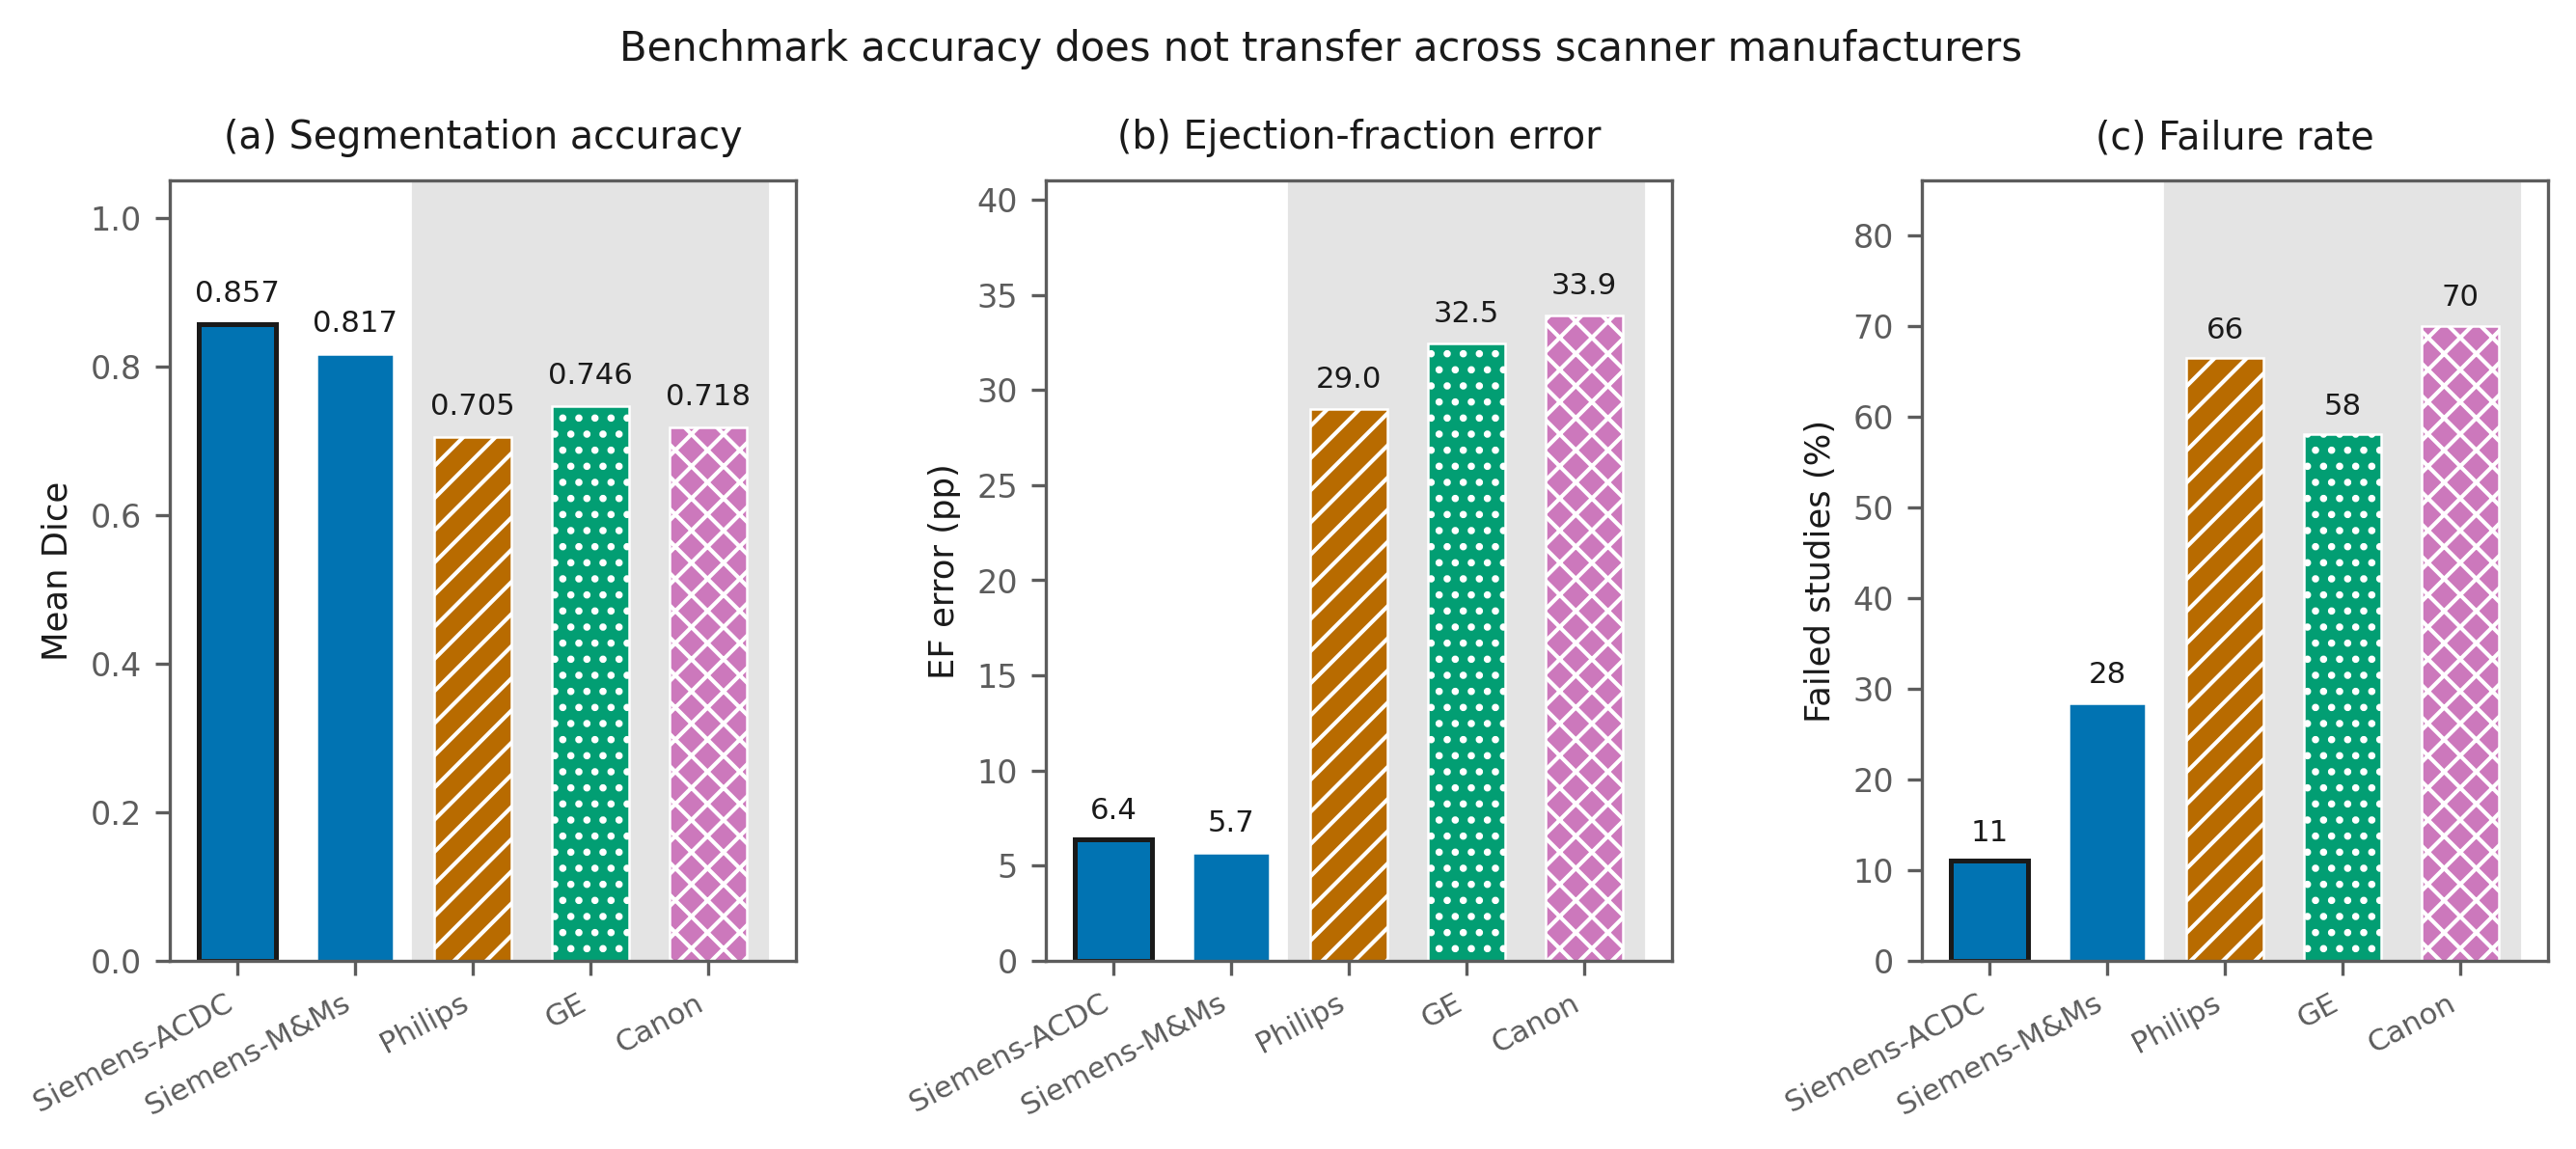
\includegraphics[width=0.9\textwidth]{figures/fig1_vendor.png}
\caption{Cross-vendor performance of the fixed segmentation system. a, Mean segmentation Dice. b, Mean absolute EF error. c, Study-level failure rate, defined as any cardiac structure with Dice $<0.70$ at an annotated phase. The shaded region denotes scanner manufacturers absent from the ACDC development cohort.}
\label{fig:vendor}
\end{figure}
\vspace{-0.6cm}

Performance varied substantially across manufacturers. EF MAE remained similar between ACDC and external Siemens examinations (6.4 versus 5.7 pp), although the failure rate increased from 11\% to 28\%. For Philips, GE, and Canon, EF MAE increased to 29.0, 32.5, and 33.9 pp, with failure rates of 66\%, 58\%, and 70\%, respectively. These changes were more pronounced than the reductions in Dice; for example, Canon LV Dice decreased from 0.858 to 0.750 while EF MAE increased from 6.4 to 33.9 pp. Thus, zero-shot inference did not ensure cross-vendor robustness, and Dice alone did not capture the effect on functional measurements, motivating study-level quality assessment. All results represent an oracle-prompt upper bound.

\subsection{Segmentation failure is detectable without ground truth}

Figure~\ref{fig:qual} illustrates the prediction-only quality signal. The left panels show the reference and predicted masks at annotated ED, allowing the true error to be visualised. The right panels show an unannotated mid-cycle frame, where both the ED- and ES-anchored masks are obtained through temporal propagation. Their disagreement map contains all pixels assigned different labels,

\begin{equation}
D(t)=
\left\{
\mathbf{p}:
M^{\mathrm{ED}}(\mathbf{p},t)
\neq
M^{\mathrm{ES}}(\mathbf{p},t)
\right\}.
\end{equation}

The Siemens example shows close inter-anchor agreement, with a \CQ{} risk of 0.12, true Dice of 0.872, and EF error of 0.2 pp. By contrast, the Canon example shows extensive disagreement, with a risk of 0.99, true Dice of 0.620, and EF error of 41.7 pp. Reference masks are displayed only for retrospective evaluation and are not used to calculate either risk score. Contours denote RV in red, myocardium in yellow, and LV in blue.

\vspace{-0.3cm}
\begin{figure}[ht]
\centering
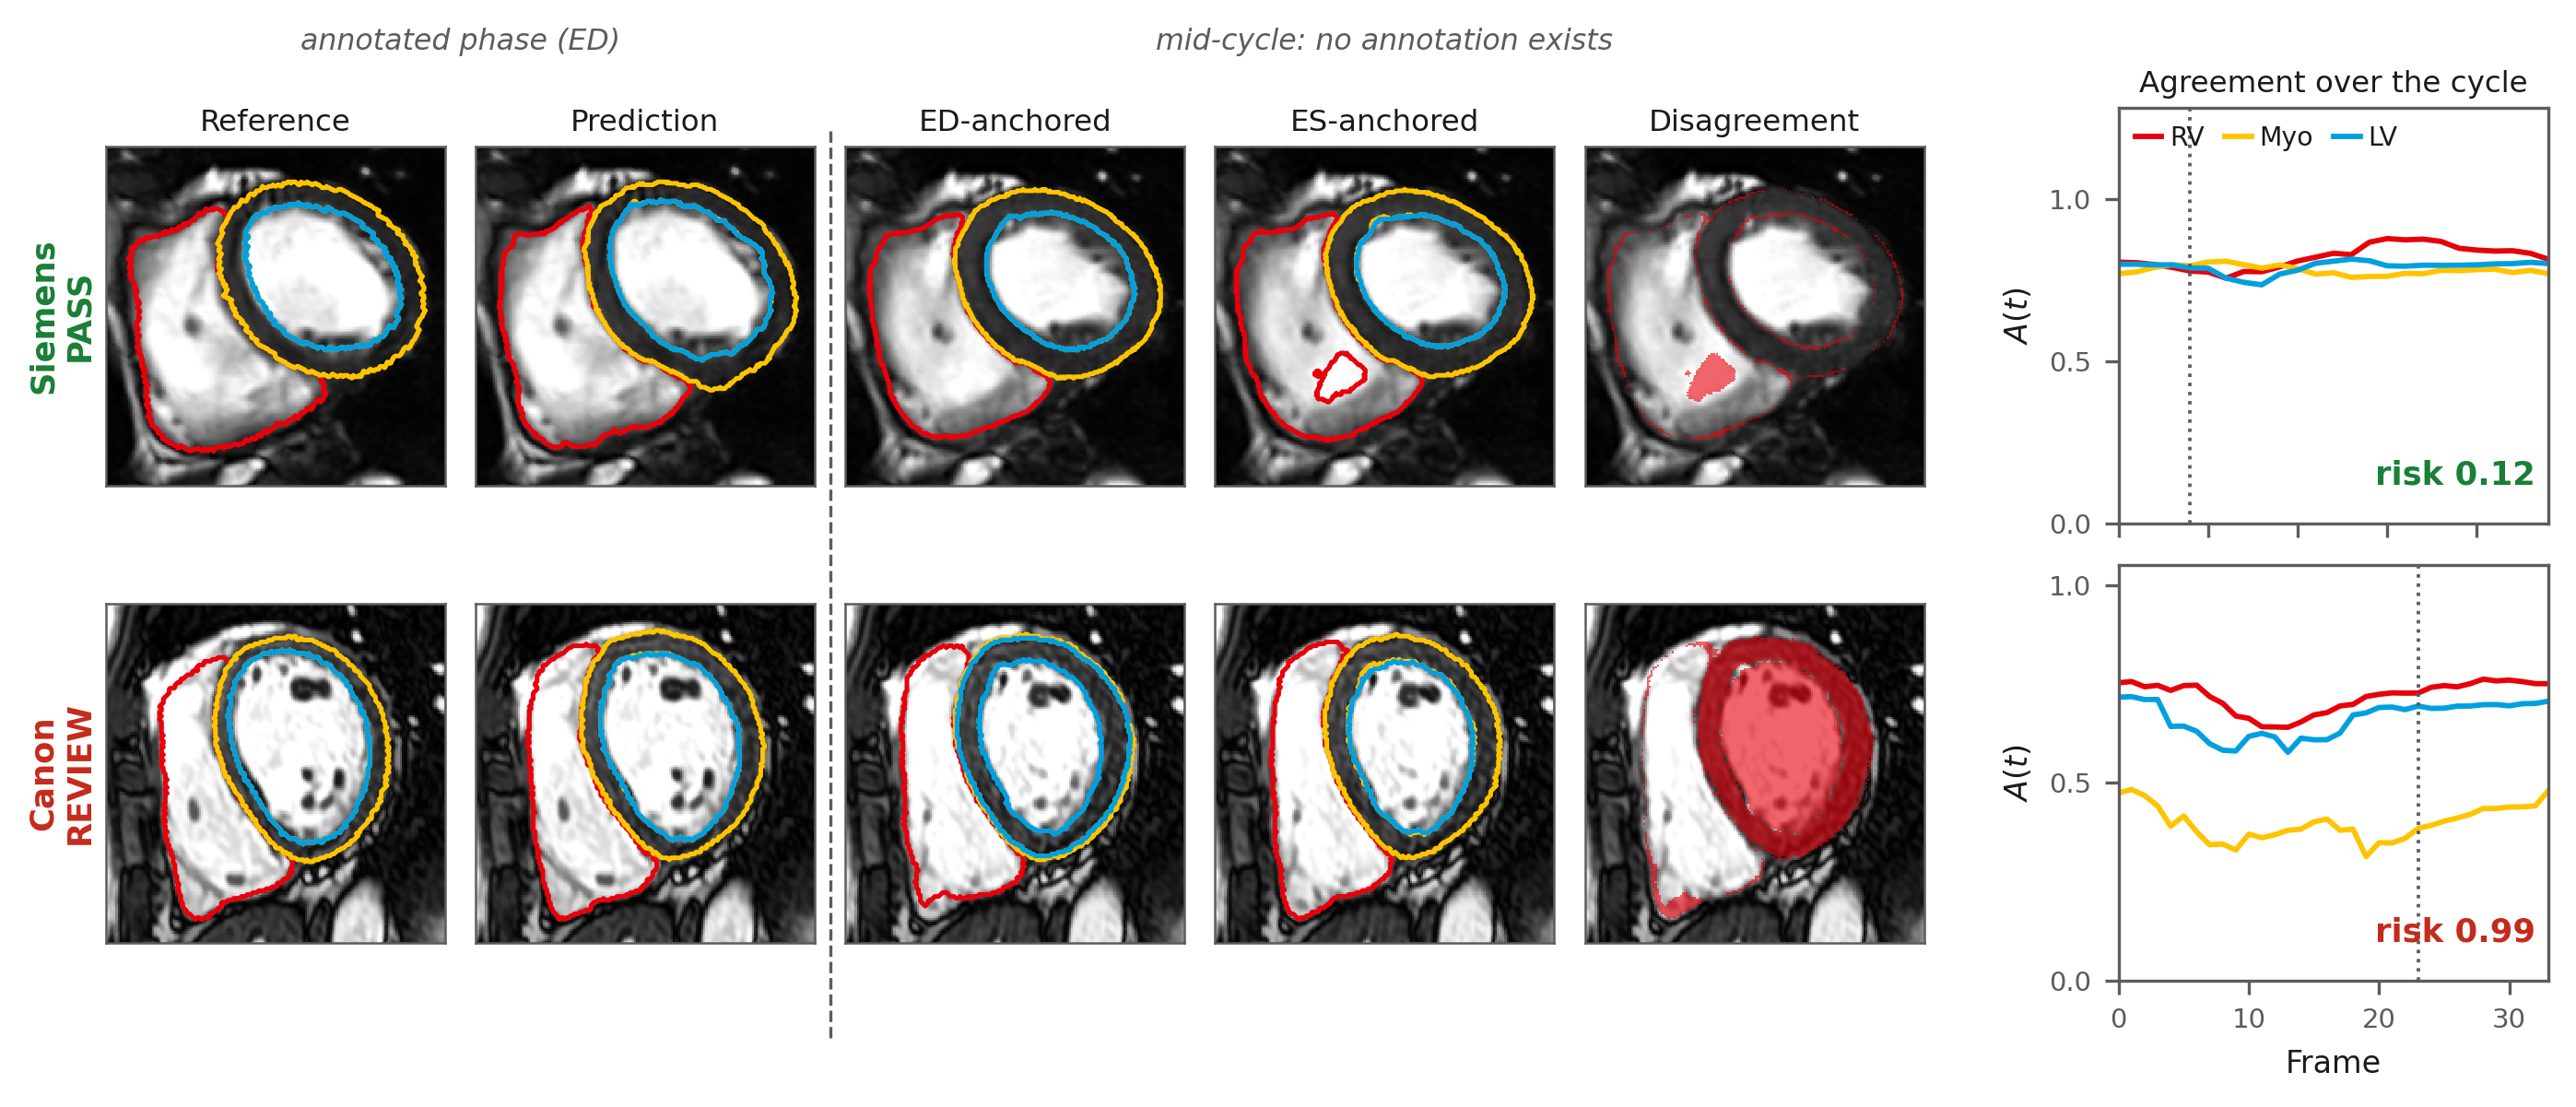
\includegraphics[width=\textwidth]{figures/fig2_qualitative.png}
\vspace{-0.5cm}
\caption{Representative low- and high-risk \CQ{} studies.}
\label{fig:qual}
\vspace{-0.8cm}
\end{figure}


Training-free quality estimation is reported in Fig.~\ref{fig:est} and Table~\ref{tab:qc} a. Without fitting a model, mean inter-anchor agreement estimated study-level Dice with an MAE of 0.064 on ACDC ($r=0.735$) and 0.072 on M\&Ms ($r=0.814$). Thus, the prediction-only agreement signal remained informative under cross-vendor domain shift.

\vspace{-0.5cm}
\begin{figure}[ht]
\centering
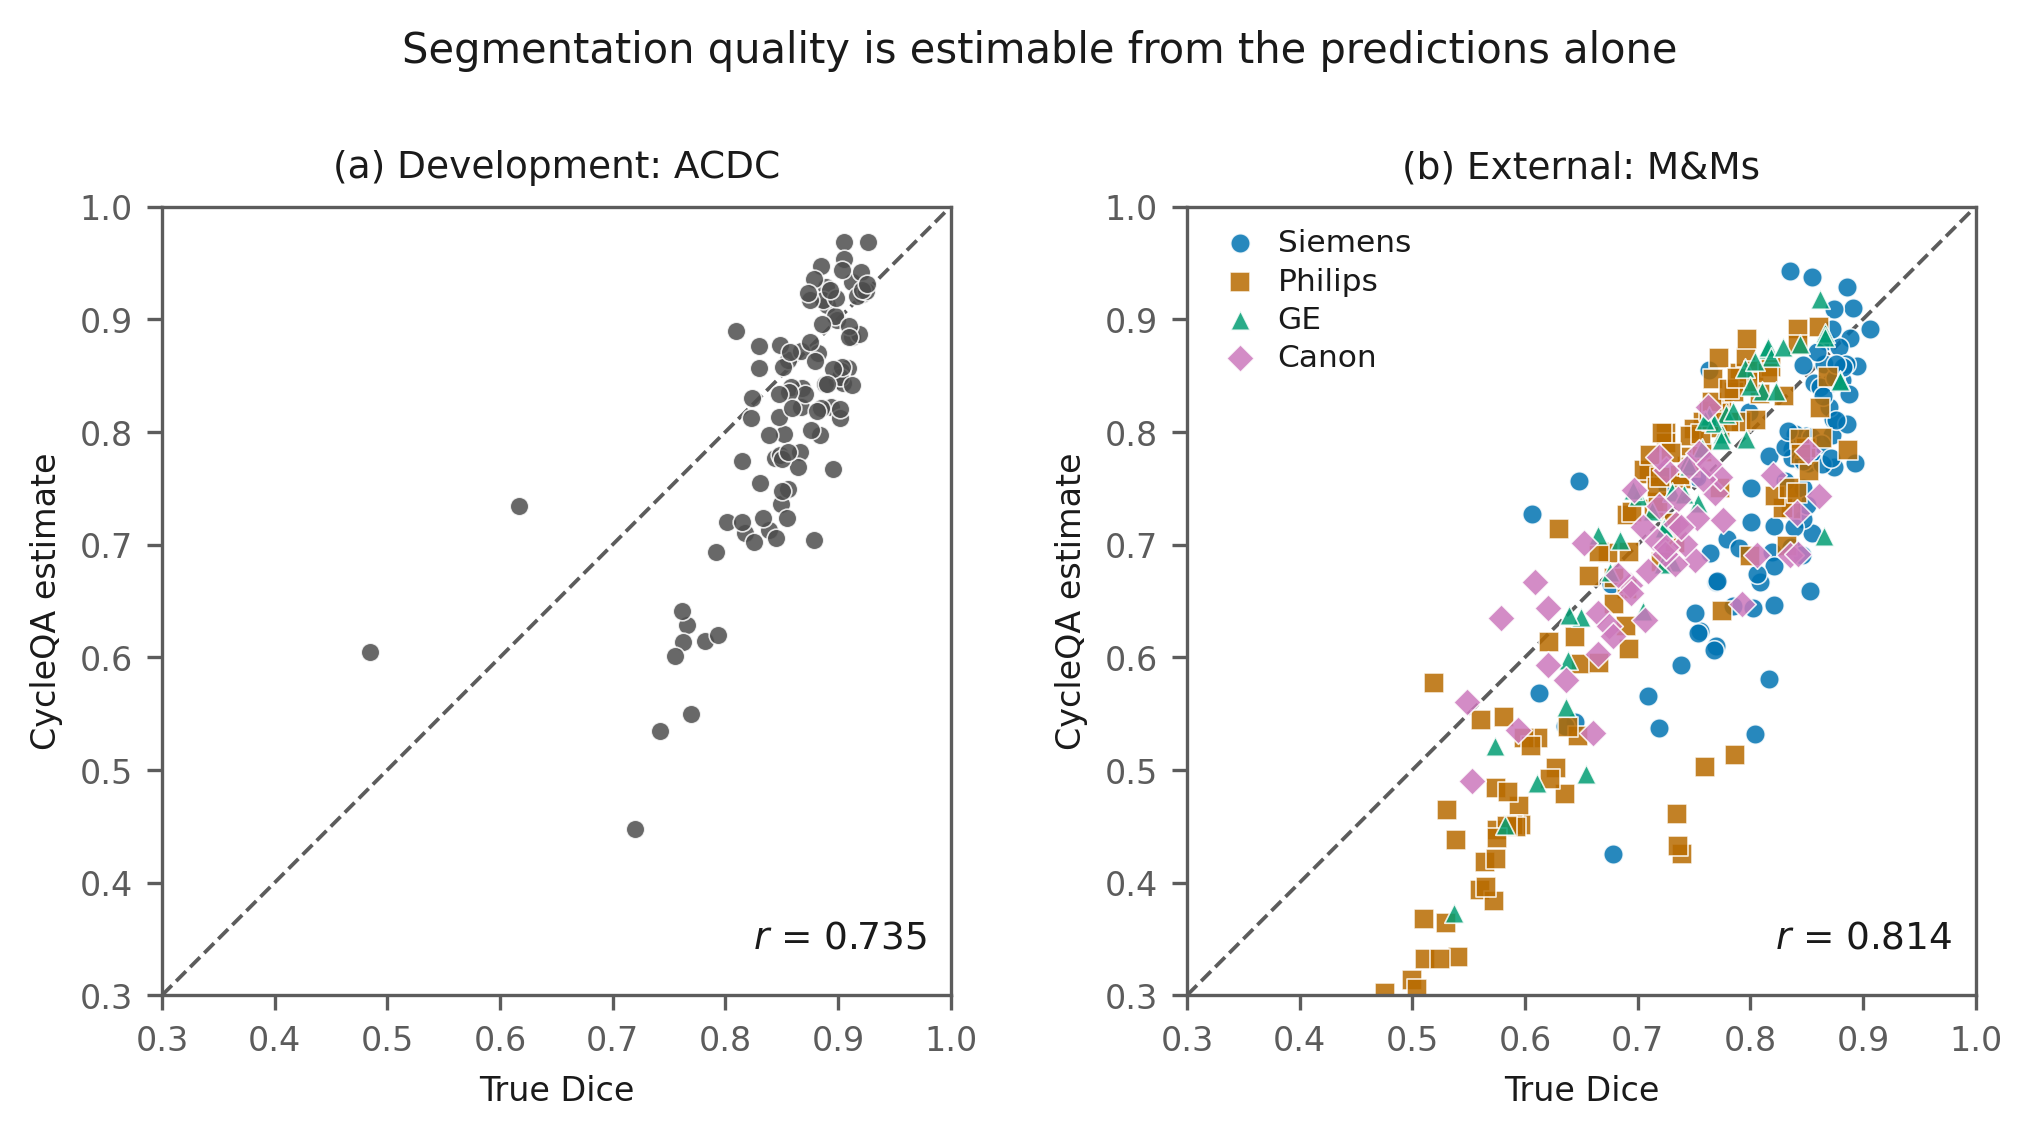
\includegraphics[width=0.8\textwidth]{figures/fig3_estimation.png}
\caption{Training-free estimation of segmentation Dice from mean inter-anchor agreement. The dashed line denotes identity.}
\label{fig:est}
\end{figure}
\vspace{-0.7cm}

The calibrated risk model achieved an external AUROC of 0.851 (95\% CI, 0.810--0.892; Fig.~\ref{fig:det}a and Table~\ref{tab:qc}b). Manufacturer-specific AUROCs were 0.883 for Siemens, 0.857 for Philips, 0.823 for GE, and 0.806 for Canon. Performance remained stable across failure definitions: varying the Dice threshold from 0.65 to 0.80 produced AUROCs of 0.823--0.894, while the secondary EF-error endpoint yielded an AUROC of 0.870. The Brier score was 0.204 (Fig.~\ref{fig:det}c).

\begin{figure}[ht]
\centering
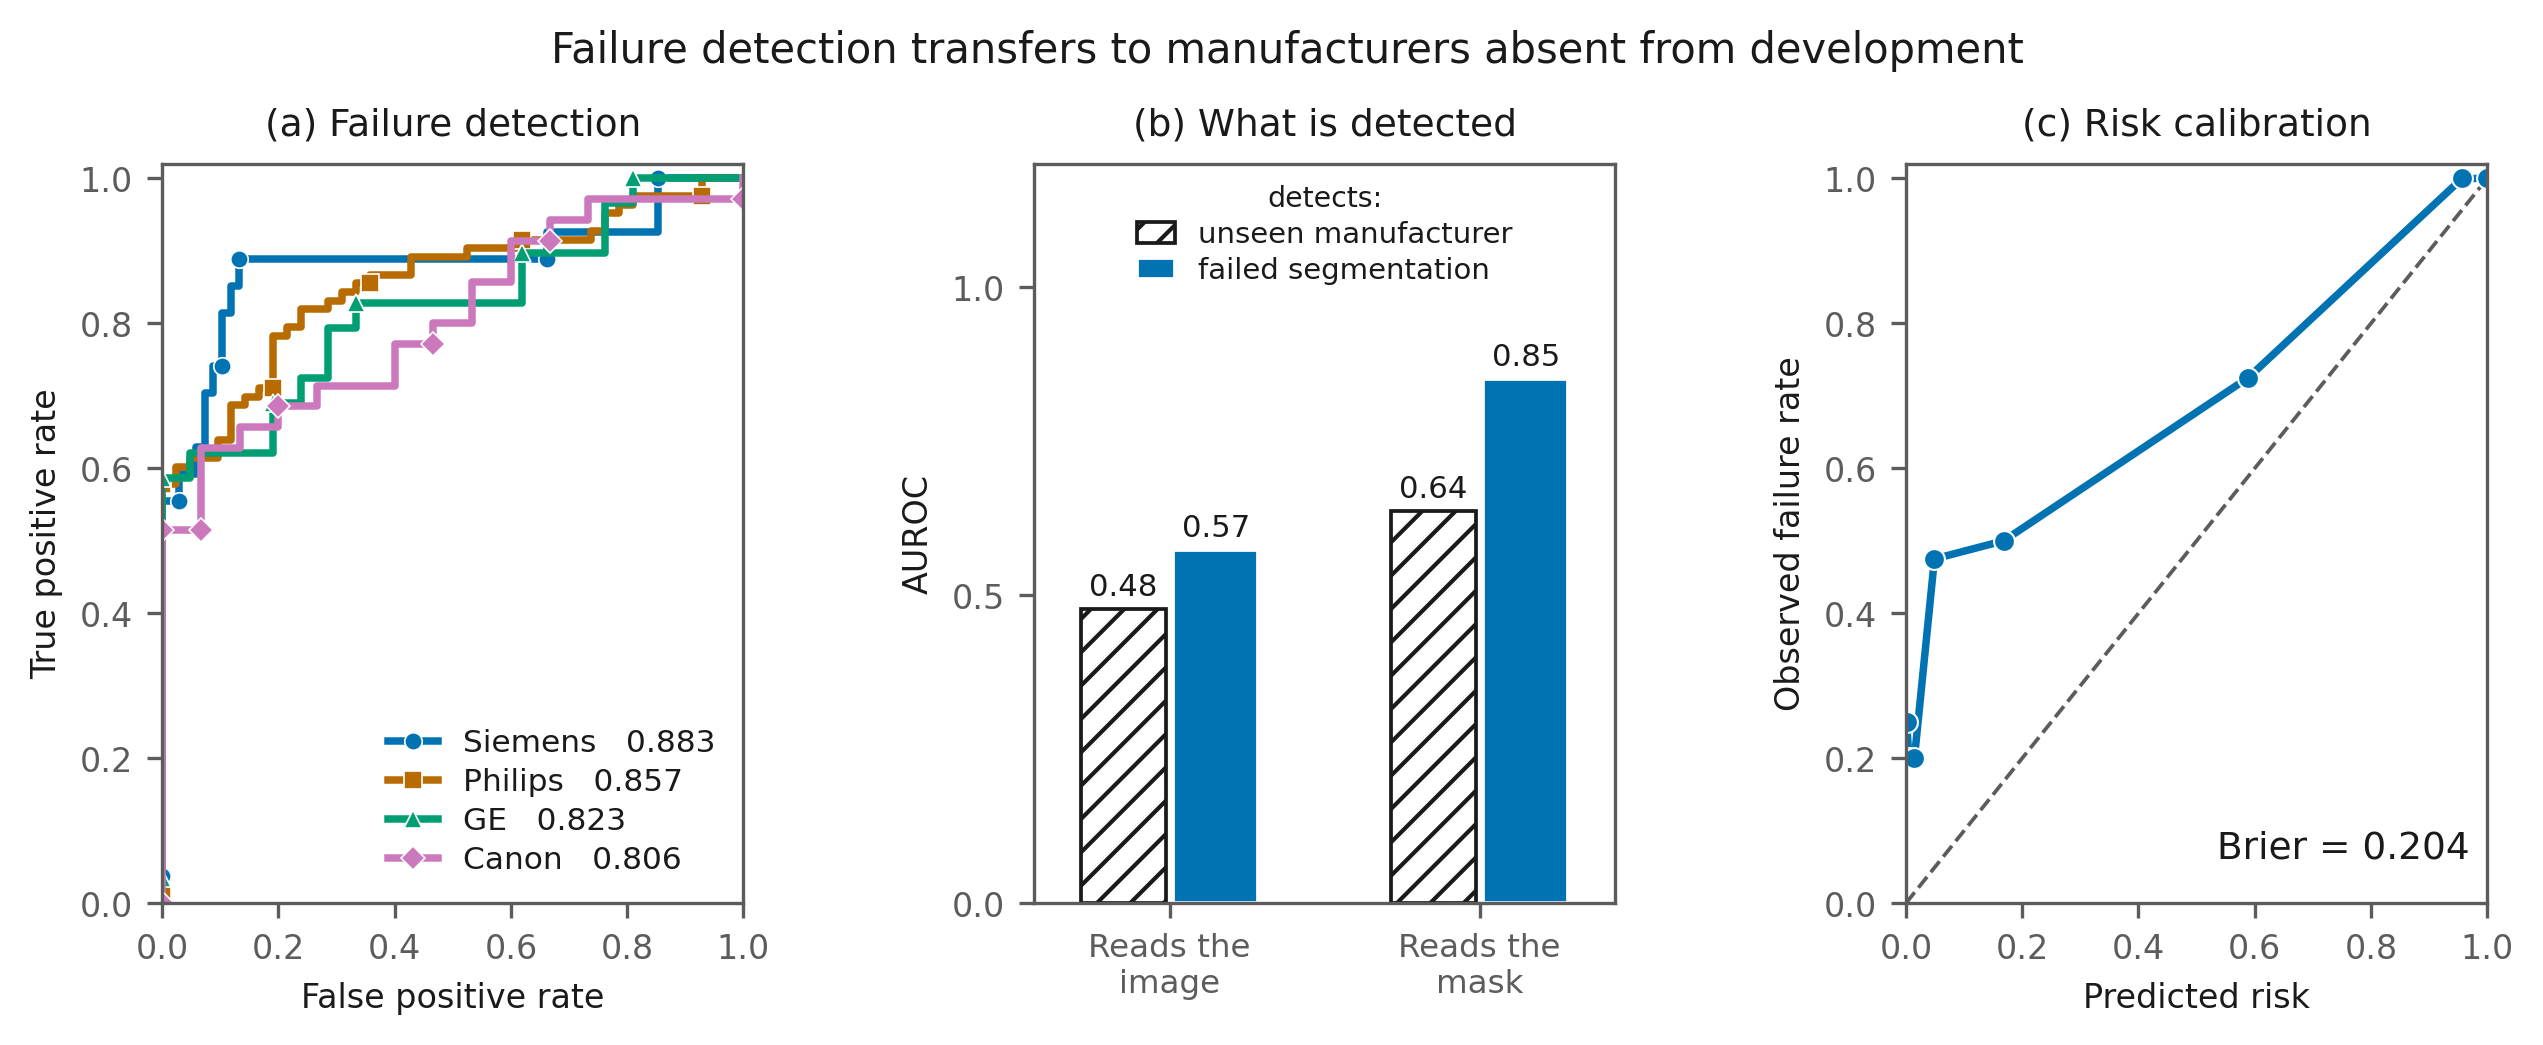
\includegraphics[width=0.9\textwidth]{figures/fig4_detection.png}
\vspace{-0.3cm}

\caption{External failure detection.Manufacturer-specific discrimination, appearance-based control, and risk calibration are shown in a-c, respectively.}
\label{fig:det}
\vspace{-0.6cm}
\end{figure}

The appearance-based control distinguished Canon examinations with an AUROC of 0.478 and detected segmentation failure with an AUROC of 0.573 (Fig.~\ref{fig:det}b). The corresponding \CQ{} AUROCs were 0.636 and 0.851. \CQ{} was therefore more strongly associated with segmentation failure than with manufacturer identity, supporting its interpretation as an output-quality signal rather than a scanner classifier.




\begin{table}[!t]
\centering
% \vspace{-0.4cm}
\caption{\CQ{} performance and ablation results.}
\label{tab:qc}
\footnotesize
\setlength{\tabcolsep}{4pt}
\renewcommand{\arraystretch}{0.98}

\begin{tabular}{@{}lccc@{}}
\toprule

\multicolumn{4}{@{}l}{\textbf{(a) Training-free Dice estimation}} \\
Cohort & $n$ & $r$ & MAE \\
\midrule
ACDC           & 100 & 0.735 & 0.064 \\
M\&Ms          & 320 & 0.814 & 0.072 \\

\midrule
\multicolumn{4}{@{}l}{\textbf{(b) Failure detection: AUROC}} \\
Method & ACDC OOF & \multicolumn{2}{c}{M\&Ms [95\% CI]} \\
\midrule
Disagreement (training-free)
    & 0.909 & \multicolumn{2}{c}{0.850 [0.811--0.888]} \\
Logistic regression
    & 0.915 & \multicolumn{2}{c}{0.851 [0.810--0.892]} \\
Random forest
    & 0.900 & \multicolumn{2}{c}{0.853 [0.808--0.892]} \\

\midrule
\multicolumn{4}{@{}l}{\textbf{(c) Feature ablation: AUROC}} \\
Feature set & $n$ & ACDC OOF & M\&Ms \\
\midrule
Anchor agreement                  & 24 & 0.987 & 0.793 \\
Plausibility                      & 22 & 0.863 & 0.891 \\
Anchor $+$ anatomical             & 30 & 0.979 & 0.789 \\
Anchor $+$ anatomical $+$ temporal
                                  & 38 & 0.959 & 0.804 \\
All feature families              & 46 & 0.915 & 0.851 \\

\midrule
\multicolumn{4}{@{}l}{\textbf{(d) Risk-guided reselection on M\&Ms}} \\
Strategy & Dice & EF MAE & Fail. (\%) \\
\midrule
Merged output             & 0.747 & 23.4 & 54.4 \\
Best fixed (post hoc)     & 0.799 & 16.8 & 21.9 \\
\textbf{\CQ{} reselection}
                          & \textbf{0.815} & \textbf{12.0} & \textbf{14.7} \\
EF-error oracle           & 0.812 & 10.4 & 17.8 \\
\bottomrule
\end{tabular}

\smallskip
\parbox{0.88\linewidth}{%
\scriptsize
OOF, out-of-fold; EF MAE is reported in percentage points.
Intervals are patient-level bootstrap 95\% CIs.
Plausibility combines anatomical, temporal, and physiological features.
}
\vspace{-0.7cm}
\end{table}


The ablation analysis revealed different internal and external behaviour (Table~\ref{tab:qc}c). A learned model using anchor-agreement features achieved an internal AUROC of 0.987 but decreased to 0.793 externally, whereas raw disagreement transferred without training at 0.850. Plausibility features alone achieved the highest external AUROC among the learned configurations (0.891), while combining all feature families yielded 0.851. These results indicate that the raw disagreement signal transfers robustly, whereas learned combinations are more sensitive to feature selection and the limited number of development failures.


Finally, risk-guided reselection improved mean Dice from 0.747 to 0.815, reduced EF MAE from 23.4 to 12.0 pp, and reduced the failure rate from 54.4\% to 14.7\% (Table~\ref{tab:qc}d). 

\subsection{Risk-guided deployment}

We first evaluated selective referral by ranking M\&Ms studies according to \CQ{} risk and withholding the highest-risk cases from automated reporting (Fig.~\ref{fig:act}a). Residual EF MAE decreased monotonically as referral coverage increased. Referring the highest-risk 20\% reduced EF MAE among the remaining studies from 23.4 to 19.8 pp. The improvement was limited by the high failure prevalence: a 20\% review budget cannot remove all failures when 54\% of studies meet the failure endpoint.
\vspace{-0.4cm}
\begin{figure}[ht]
\centering
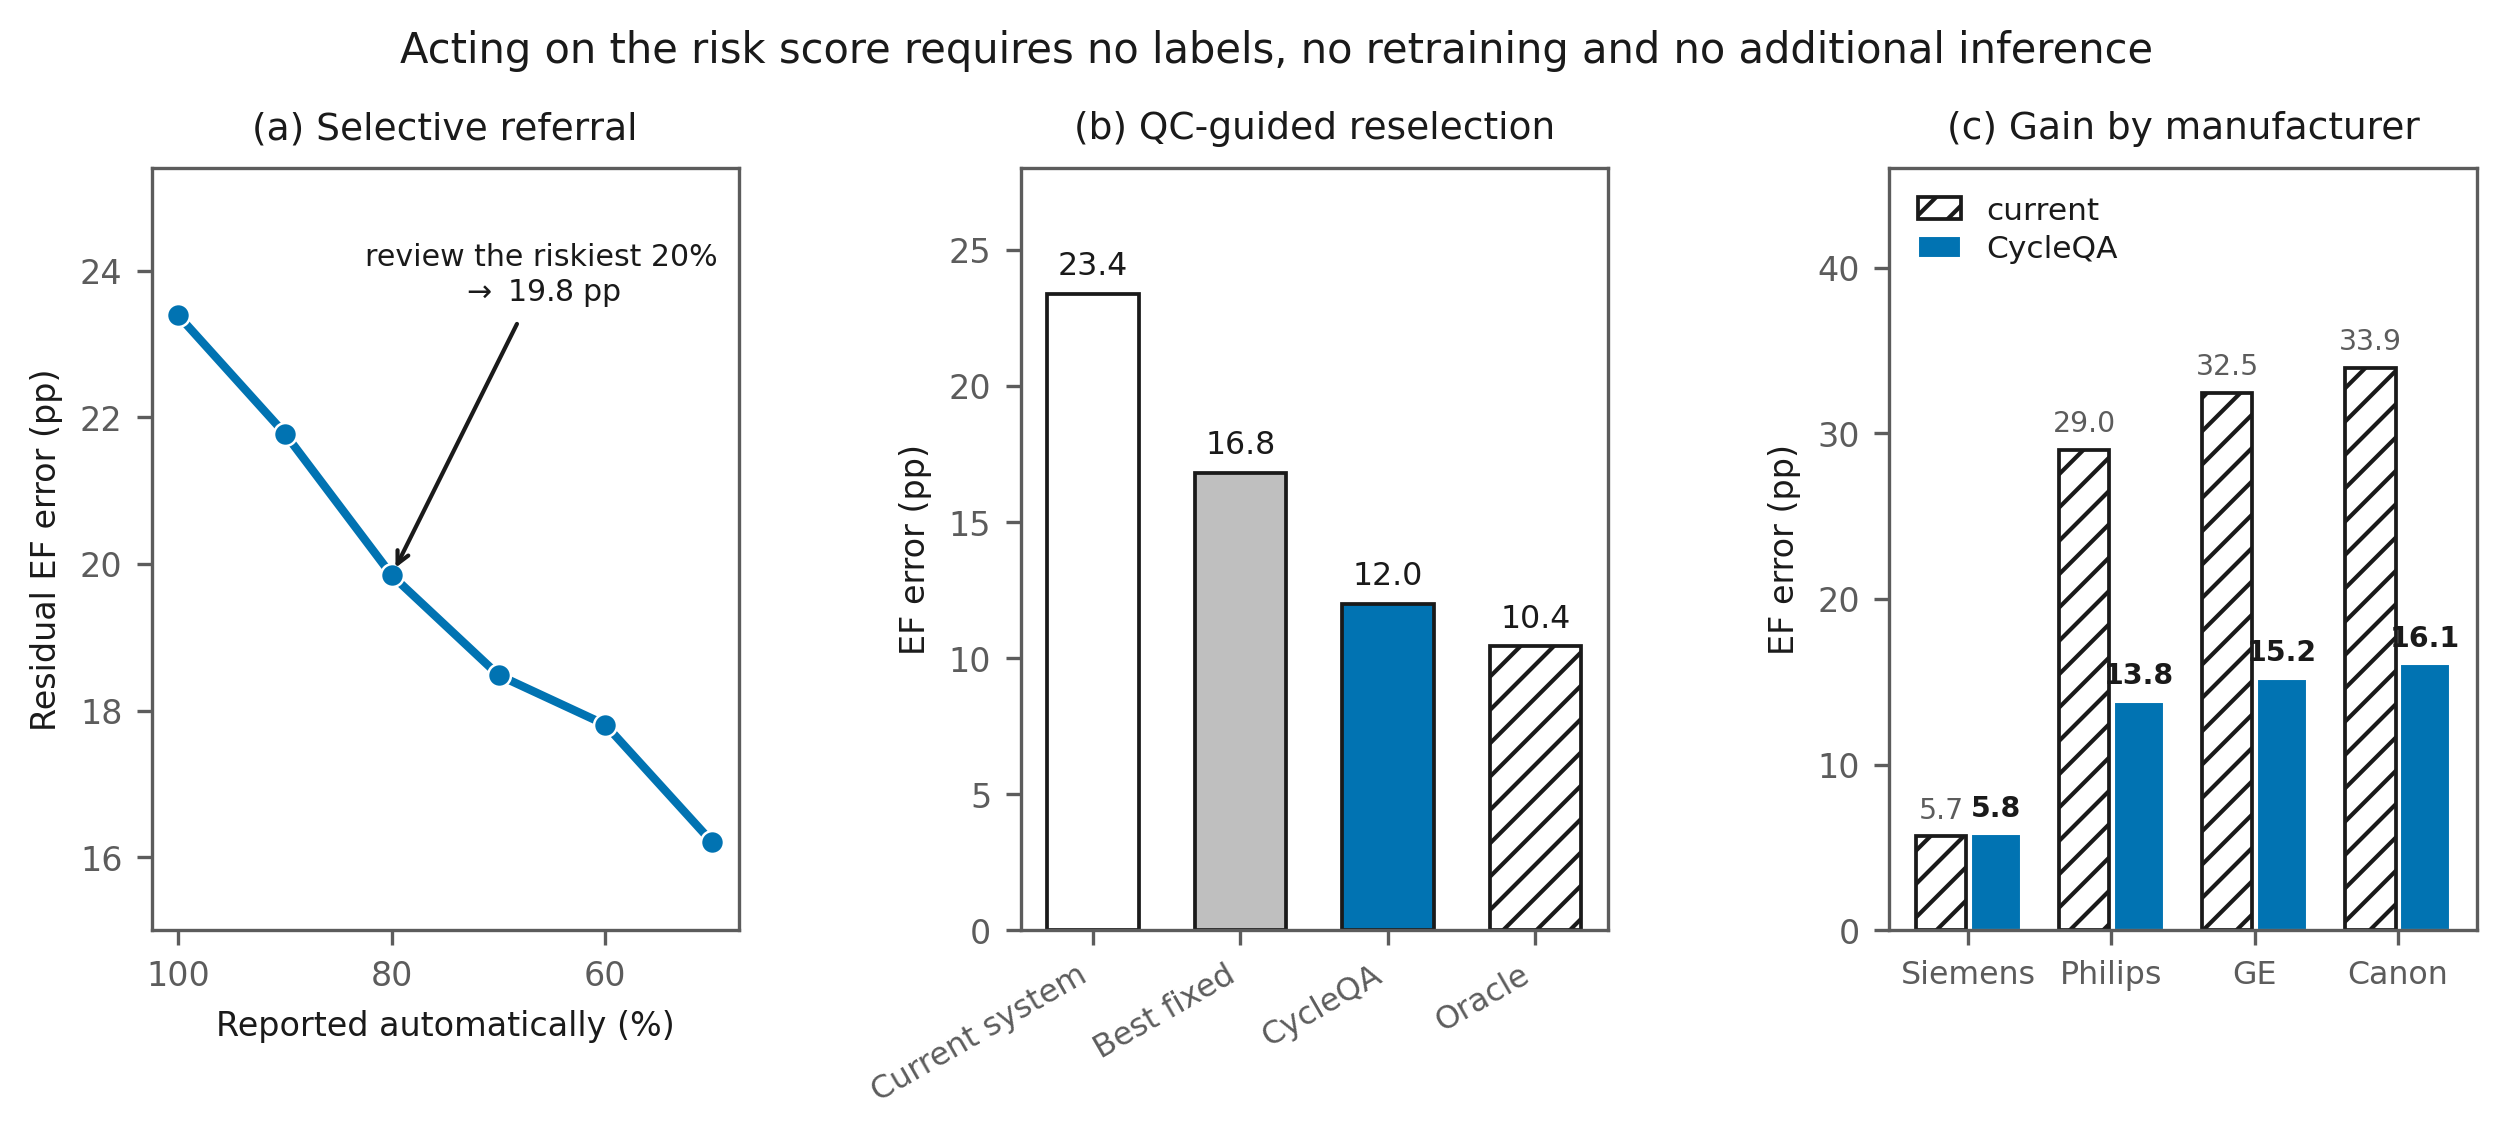
\includegraphics[width=\textwidth]{figures/fig5_action.png}
\caption{Risk-guided deployment on the external M\&Ms cohort. a, Selective referral. b, Prediction reselection. c, Manufacturer-specific selection patterns.}
\label{fig:act}
\end{figure}

\vspace{-0.5cm}
We next used \CQ{} to select among the ED-anchored, ES-anchored, and merged predictions already generated for each study (Fig.~\ref{fig:act}b and Table~\ref{tab:qc}d). The preferred prediction differed across datasets: the merged output performed best on ACDC, whereas the ES-anchored output was the best fixed choice on M\&Ms, reducing EF MAE from 23.4 to 16.8 pp. However, identifying this fixed choice requires external labels. In contrast, \CQ{} selected the lowest-risk prediction independently for each study, reducing EF MAE to 12.0 pp and the failure rate from 54.4\% to 14.7\%. The resulting EF error approached the reference-based oracle of 10.4 pp and was lower than the post hoc best fixed strategy. Reselection required no target-domain labels, model retraining, or additional segmentation inference.

Selection patterns varied across manufacturers (Fig.~\ref{fig:act}c). For Siemens examinations, \CQ{} retained the merged or ED-anchored prediction in 92\% of studies and achieved an EF MAE of 5.8 pp; always selecting the ES-anchored prediction would have increased it to 14.8 pp. For Philips, GE, and Canon, \CQ{} selected the ES-anchored prediction more frequently. Thus, no single fixed strategy performed consistently across manufacturers, whereas \CQ{} adapted the selection at the study level without using manufacturer information.

\section{Discussion and Conclusion}

This study shows that zero-shot segmentation does not ensure cross-vendor robustness. On M\&Ms, EF MAE increased from 6.4 to 23.4 pp and the failure rate from 11\% to 54\%, despite smaller changes in Dice. \CQ{} remained informative because it assesses consistency and plausibility from predicted masks rather than scanner appearance. Inter-anchor agreement does not guarantee correctness, as both predictions may share the same error, but it provides a useful signal of propagation instability.

\CQ{} converts this signal into practical intervention. Selective referral prioritises high-risk studies for review, while risk-guided reselection chooses among predictions already generated by the segmentation system. Reselection reduced EF MAE from 23.4 to 12.0 pp and the failure rate from 54.4\% to 14.7\%, without target-domain labels, retraining, or additional segmentation inference.

This study has several limitations. Reference-derived prompts make the results an oracle-prompt upper bound, and automatic prompt generation remains necessary for deployment. Reference masks were available only at ED and ES, preventing direct validation at intermediate phases. Evaluation was retrospective, and the small development cohort limited the stability of learned risk models. Supervised baselines were excluded because their checkpoint provenance could not be verified. Nevertheless, training-free disagreement estimated external Dice with an MAE of 0.072 and detected failed studies with an AUROC of 0.850. These results support prediction-only quality assessment \CQ{} as a practical safeguard for zero-shot cine CMR segmentation under domain shift.
% \section{Discussion}

% \subsubsection{Why quality assurance transfers when segmentation does not.}
% The segmentation model must answer a hard question---\emph{which pixels are myocardium?}---and
% to do so it must read appearance. Appearance is what changes between scanners, so the model
% breaks. \CQ{} asks two easy questions: \emph{are you consistent with yourself?} and \emph{is
% your answer anatomically possible?} Neither requires the image. A heart is a heart on any
% scanner: the myocardium encloses the LV cavity, the volume curve closes, EDV exceeds ESV.
% These constraints are vendor-invariant \emph{by construction}, which is why a detector built
% on them survives a change of manufacturer that the segmenter does not. Verifying an answer
% is easier than producing it---and so the watchdog is more robust than the model it watches.

% \subsubsection{Deployment and post-market surveillance.}
% A site installs the tool with no labels and no retraining. Every study receives a \CQ{} score
% in about a second of CPU time, with no second network. Studies below threshold are
% auto-reported; high-risk studies are flagged for review, with the risk--coverage curve
% converting review capacity into a budgeted decision; and where a more plausible alternative
% propagation exists, it is substituted automatically. Beyond the individual study, the
% \emph{mean} \CQ{} risk across a site's workload is itself a label-free proxy for
% performance: a drift above the development baseline is an alarm that the site is out of
% distribution, raised before any patient has been misreported. Regulators require
% post-market surveillance of deployed AI devices, and the usual obstacle is that the real
% world supplies no ground truth. \CQ{} supplies a surrogate.

% \subsubsection{Limitations.}
% Prompts are derived from reference masks, so our numbers are an oracle-prompt upper bound;
% real deployment additionally needs automatic prompt generation. Reference masks exist only
% at ED and ES, so we validate annotated-phase error and make no claim about intermediate
% phases. Evaluation is retrospective and on public data; there is no prospective clinical
% validation. The review threshold is an operating choice each site must set against its own
% risk tolerance. Finally, the development set (100 patients, 11 failures) is small---which is
% precisely why the training-free tier, not the learned one, is our recommended configuration.
% Supervised U-Net and DINOv2 baselines were also run on M\&Ms, but the provenance of their
% training checkpoints could not be established with certainty, so they are excluded rather than
% reported as a comparison that cannot be defended.


% \section{Conclusion}

% A zero-shot cardiac video foundation model that scores 0.91 Dice on a public benchmark
% produces a 34-point ejection-fraction error on an unseen scanner---and at that site there is
% no ground truth with which to notice. We showed the failure is legible from the predicted
% masks alone, because dual-anchored propagation runs the same video twice and the two passes
% disagree exactly when the model is wrong. Used without any training, that disagreement
% estimates Dice to within 0.072 and detects failed studies at AUROC 0.850 on manufacturers
% absent from development; used to reselect among predictions already computed, it halves
% ejection-fraction error. The redundancy introduced to make the model accurate is the
% redundancy that makes it self-auditing. A fragile model can be deployed safely if the
% watchdog watching it is not fragile.

\bibliographystyle{splncs04}
\bibliography{references}

\end{document}
